\documentclass{article}
\usepackage{ctex}
\usepackage{graphicx}
\usepackage{float}
\usepackage{geometry}
\usepackage{amssymb}
\usepackage{amsmath}
\usepackage{multirow}

%opening
\title{文泉考试平台 开发文档}
\author{200 OK}
\date{}
\geometry{a4paper, left=3.18cm, right=3.18cm, top=2.54cm, bottom=2.54cm}

\begin{document}

\maketitle

\section{需求分析}
    \subsection{用户管理}
        \begin{enumerate}
         \item 用户类型包括以下三种:超级管理员、管理员、学员
            \begin{itemize}
             \item 不同用户类型具有不同权限,同一页面显示内容应当根据用户权限改变。
            \end{itemize}
        \item 用户管理页面向管理员以列表形式呈现用户属性,包括用户名、类型、邮箱、最近登录IP
            \begin{itemize}
             \item 只有管理员可以进入用户管理页面;
             \item 其他用户尝试进入用户管理页面(如输入$url$)需有错误提示。
            \end{itemize}
        \item 管理员可创建、查看、编辑、封禁用户。
            \begin{itemize}
             \item 用户管理页面需添加按钮使管理员对用户进行创建、查看、编辑、封禁、解禁操作;
             \item 创建用户提供用户名、密码、邮箱、用户类型,且用户类型不能为超级管理员;
             \item 查看用户内容包括用户名、类型、邮箱、最近登录IP;
             \item 编辑用户内容包括将学生权限提升;
             \item 封禁用户后用户不能正常登录,并且在登录页面有错误提示;
             \item 管理员可以封禁学生,超级管理员可以封禁管理员,管理员不能封禁管理员。
            \end{itemize}
        \item 管理员由超级管理员创建,学员使用邮箱自行注册,通过邮箱激活。
            \begin{itemize}
             \item 超级管理员即$root$,只能伴随系统产生,只有一个,不能有其他途径创建;
             \item 管理员只能由超级管理员创建,或被从学生提升为管理员;
             \item 学员之间的区分以邮箱作为唯一标识,注册时需要对邮箱是否已注册进行检验;
             \item 学员成功注册后给相应邮箱发送邮件,包含导航至验证成功提示的页面的链接。
            \end{itemize}
        \end{enumerate}
        \begin{figure}[H]
            \centering
            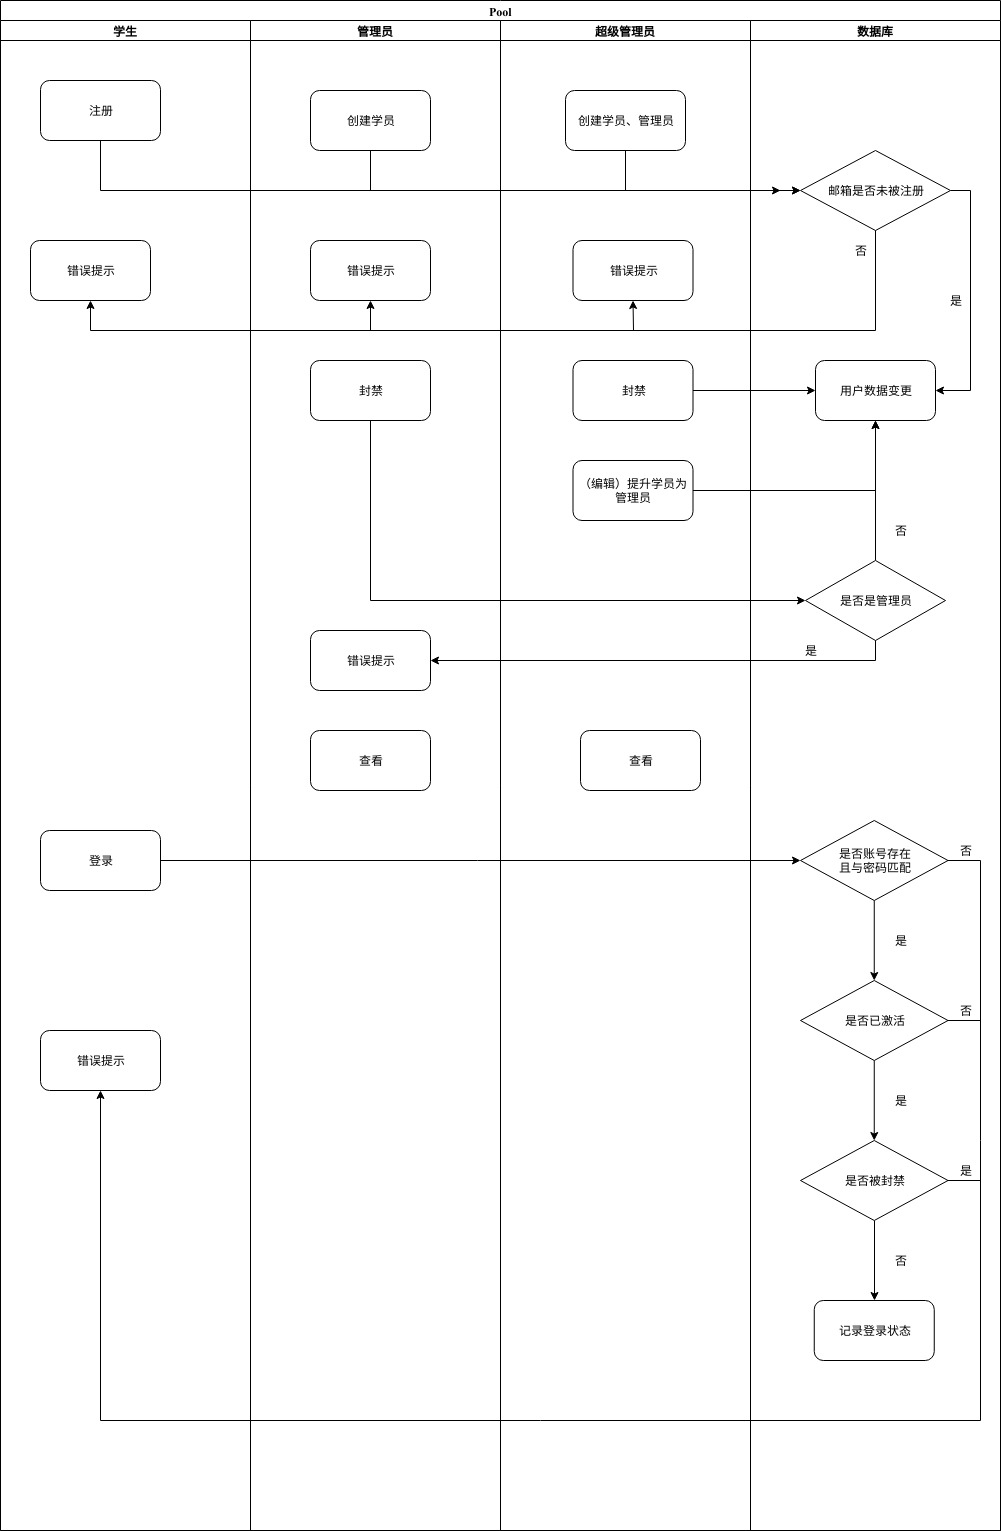
\includegraphics[width=.8\textwidth]{./UserManageMent.jpg}
        \end{figure}

    \subsection{题库管理}
    
    \subsection{学习系统}
    	\begin{enumerate}
    		\item 在登陆之后,学生可以选择题库开始学习。
    		\item 学习系统分为两个板块:自主练习、试卷模考。
    		\item 进入自主练习模块后,学生可以选择知识点练习该题库下的题目。
    		\begin{itemize}
    			\item 学生需要先选择题库后才能继续;
    			\item 输入习题数量之后,系统从题库中抽取对应数量的题目,然后开始练习;
    			\item 答题完毕后显示答案对错与题目解析;
    			\item 题目抽取时不抽取主观题。
    		\end{itemize}
   			\item 进入试卷模考模块后,学生可以完成后台试卷管理创建的试卷。
   			\begin{itemize}
   				\item 试卷完成后系统批阅客观题,主观题提交到后台等待批阅;
   				\item 试卷完成后直接显示客观题批阅结果;
   				\item 试卷批阅完成后在查看试卷时显示评分和批语。
   			\end{itemize}
    	\end{enumerate}
    \subsection{非功能需求}
		\begin{enumerate}
			\item 平台界面设计合理、逻辑清晰。
			\item 平台能兼容电脑、手机和平板等终端浏览器浏览。
			\item 对用户易于学习和使用,用户体验友好。
			\item 根据用户权限控制访问数据,进行操作记录。
			\item 系统出错时,不影响用户的行为操作与数据。
		\end{enumerate}
\end{document}

